\chapter{Het zonnestelsel}\label{ch:g4:solar-system}

De Aarde legt, zoals je weet, elk jaar een ronde om de Zon af. Maar
reist ze alleen? Kijk op een heldere avond omhoog: tussen de vaste
fonkelingen dwalen een paar heldere lichtjes van week tot week
langzaam rond. De ouden noemden ze de dwalers; wij noemen ze
planeten --- werelden die om dezelfde Zon draaien als wij.

\section{Eén ster, acht planeten}

\begin{definition}[Ster]\label{def:g4:solar-system:star}
Een \emph{ster}\index{ster} is een reusachtige bal gloeiend hete stof
die zijn eigen \omterm{def:g1:light-and-shadows:source}{licht} maakt --- een echte \omterm{def:g1:light-and-shadows:source}{lichtbron}. De Zon is een ster:
onze ster, dicht genoeg bij om ons gezicht te verwarmen. (De andere
sterren van de nacht krijgen volgend jaar een eigen hoofdstuk.)
\end{definition}

\begin{definition}[Planeet]\label{def:g4:solar-system:planet}
Een \emph{planeet}\index{planeet} is een grote, ronde wereld die om
een \omterm{def:g4:solar-system:star}{ster} reist en geen eigen \omterm{def:g1:light-and-shadows:source}{licht} maakt --- we zien planeten, net
als de \omterm{def:g2:moon-in-the-sky:moon}{Maan}, door het zonlicht dat ze terugsturen. De Aarde is een
planeet.
\end{definition}

\begin{definition}[Het zonnestelsel]\label{def:g4:solar-system:family}
Het \emph{zonnestelsel}\index{zonnestelsel} is de Zon samen met alles
wat om haar heen reist: de acht planeten --- op volgorde: Mercurius,
Venus, Aarde, Mars, Jupiter, Saturnus, Uranus, Neptunus --- plus hun
manen en een menigte kleinere rotsen en ijsballen.
\end{definition}

\begin{omfigure}
\begin{tikzpicture}[scale=0.85]
  % the Sun, anchored in the corner
  \fill[omThm] (0,0) -- (0.65,0) arc (0:40:0.65) -- cycle;
  \node[below, font=\small] at (0.45,-0.95) {de Zon};
  % one generous arc of each orbit
  \foreach \r in {1.3, 2.1, 2.9, 3.7, 5.2, 6.9, 8.5, 10.1} {
    \draw[dashed, omExo] (\r,0) arc (0:40:\r);
  }
  % the planets, labels staggered in two rows
  \foreach \r/\name in {1.3/Mercurius, 2.9/Aarde, 5.2/Jupiter,
      8.5/Uranus} {
    \fill[omDef] (\r,0) circle (0.11);
    \node[below, font=\footnotesize] at (\r,-0.18) {\name};
  }
  \foreach \r/\name in {2.1/Venus, 3.7/Mars, 6.9/Saturnus,
      10.1/Neptunus} {
    \fill[omDef] (\r,0) circle (0.11);
    \draw[omExo, very thin] (\r,-0.18) -- (\r,-0.72);
    \node[below, font=\footnotesize] at (\r,-0.75) {\name};
  }
\end{tikzpicture}

{\small De Zon en haar acht planeten, op volgorde --- hier schouder aan
schouder getekend, terwijl in werkelijkheid elke baan ver, heel ver
voorbij de vorige ligt.}
\end{omfigure}

\begin{proposition}[De gewoonten van de planeten]\label{prop:g4:solar-system:habits}
De planeten houden er nette gewoonten op na: elk reist om de Zon over
zijn eigen bijna cirkelvormige weg, ze draaien allemaal dezelfde kant
op, en al die wegen liggen bijna in één plat vlak --- als ringen
getekend op één tafelblad. En hoe verder de weg van een \omterm{def:g4:solar-system:planet}{planeet} van
de Zon ligt, hoe langer één ronde duurt: Mercurius doet er $88$ dagen
over, de Aarde één jaar, het verre Neptunus $165$ jaar.
\end{proposition}

\begin{example}[Rotsplaneten en gasreuzen]\label{ex:g4:solar-system:kinds}
De vier binnenste planeten --- Mercurius, Venus, Aarde, Mars --- zijn
ballen van gesteente, klein en vast: werelden waarop je zou kunnen
staan. De vier buitenste --- Jupiter, Saturnus, Uranus, Neptunus ---
zijn de \emph{reuzen}: enorme ballen die vooral uit dik \omterm{def:g3:solids-liquids-gases:gas}{gas} bestaan,
zonder enige grond om op te staan. Jupiter, de grootste, zou meer dan
duizend Aardes kunnen opslokken; Saturnus draagt zijn beroemde
glanzende ringen --- ontelbare stukjes ijs die als een menigte
piepkleine manen om hem heen cirkelen.
\end{example}

\begin{omfigure}
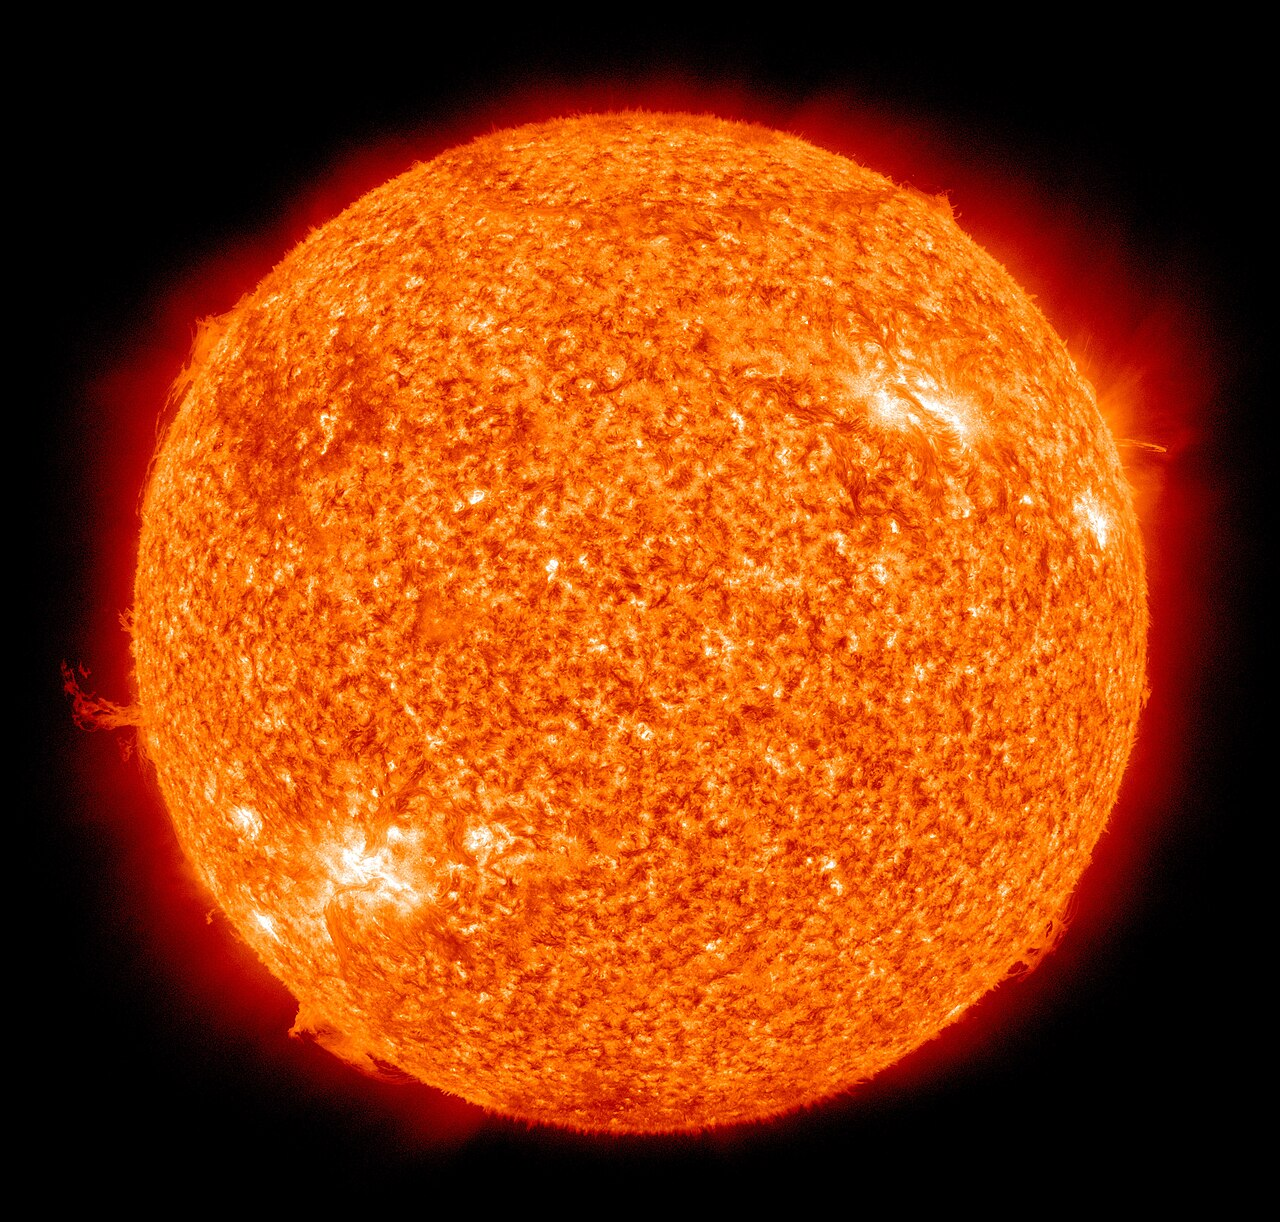
\includegraphics[height=3.1cm]{images/book1/sun-sdo.jpg}

{\small de Zon, onze \omterm{def:g4:solar-system:star}{ster}}

\medskip
\begin{tabular}{cccc}
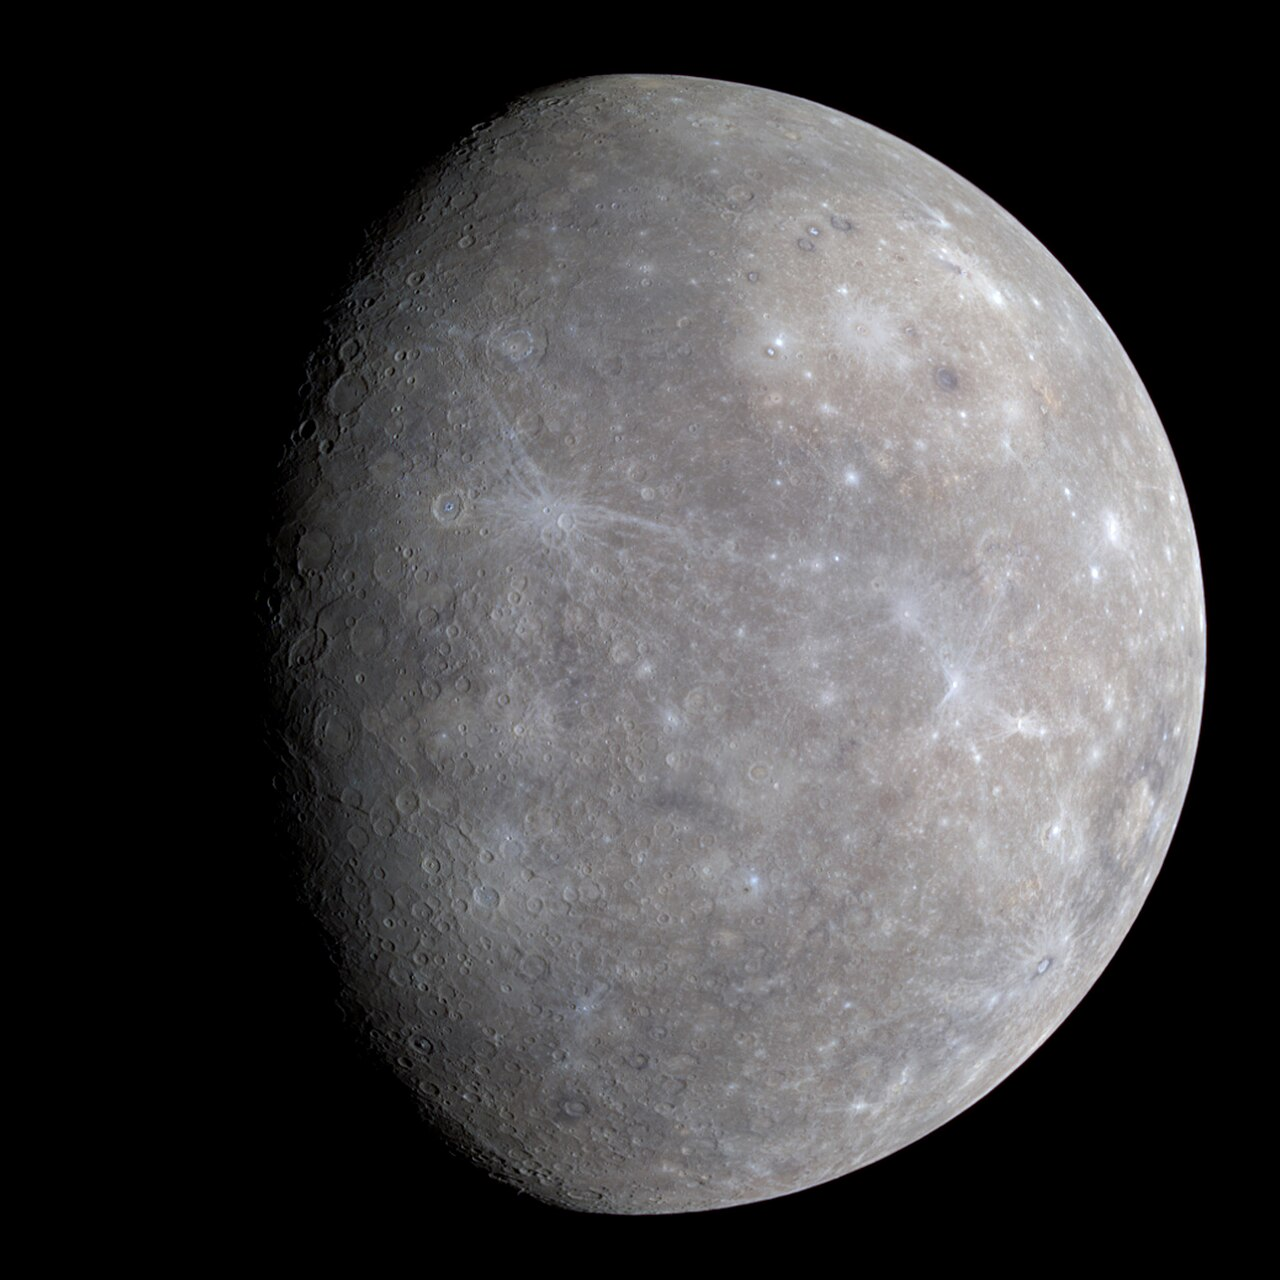
\includegraphics[height=1.75cm]{images/book1/mercury.jpg} &
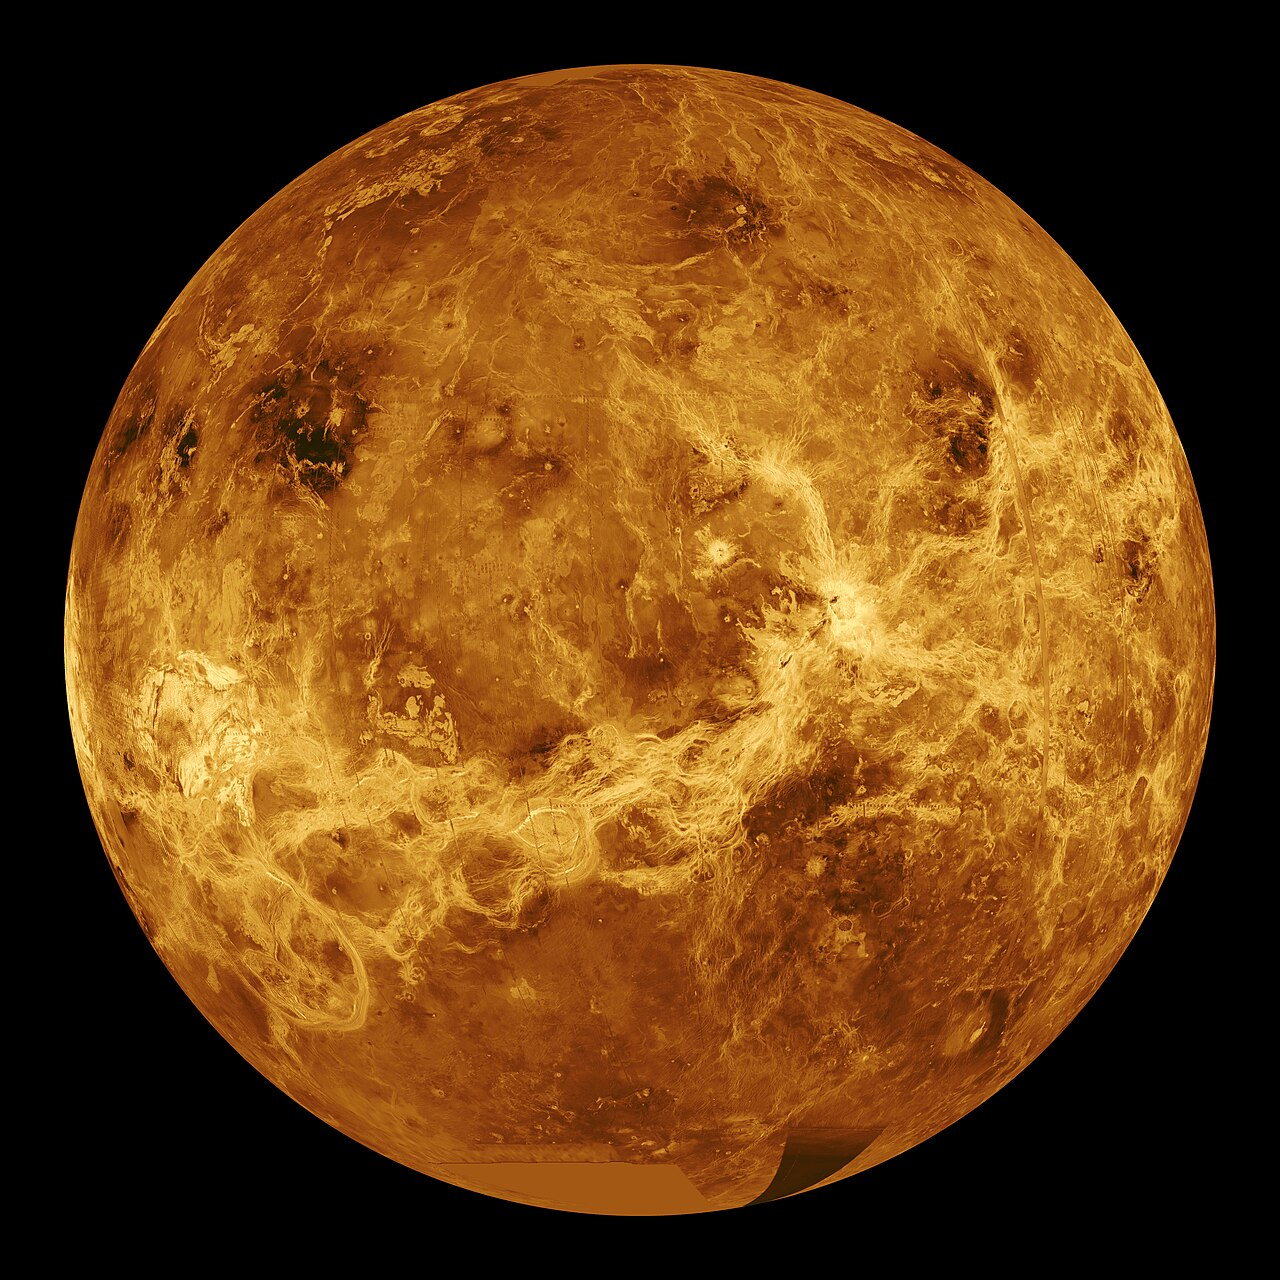
\includegraphics[height=1.75cm]{images/book1/venus.jpg} &
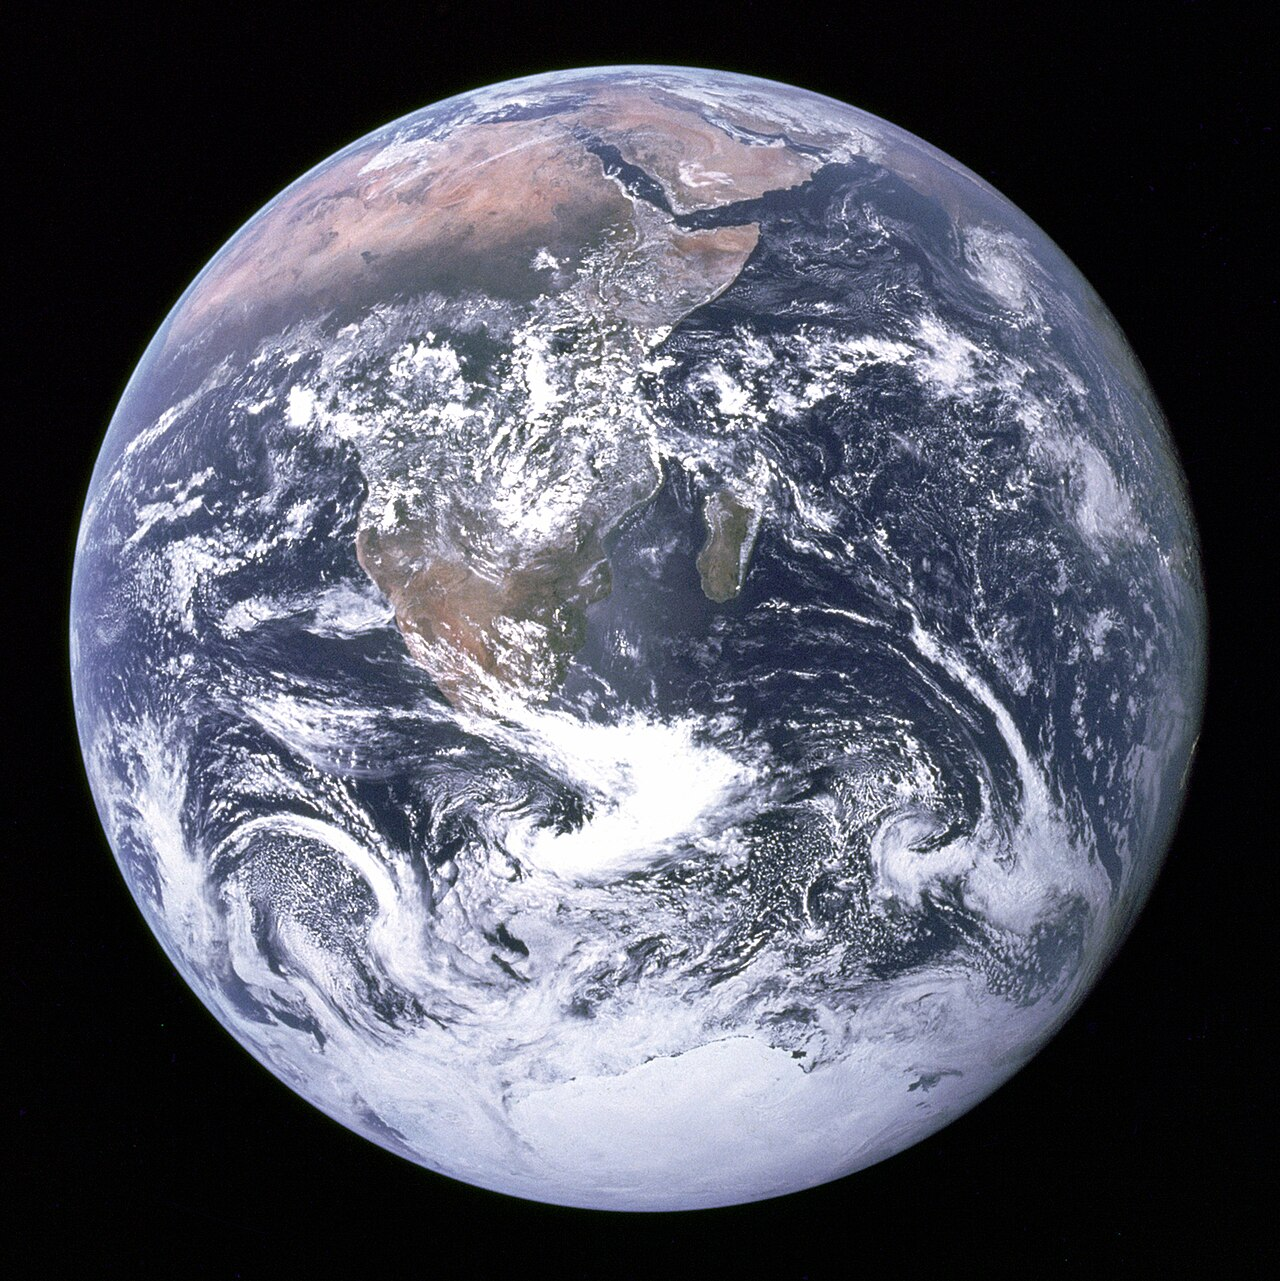
\includegraphics[height=1.75cm]{images/book1/earth.jpg} &
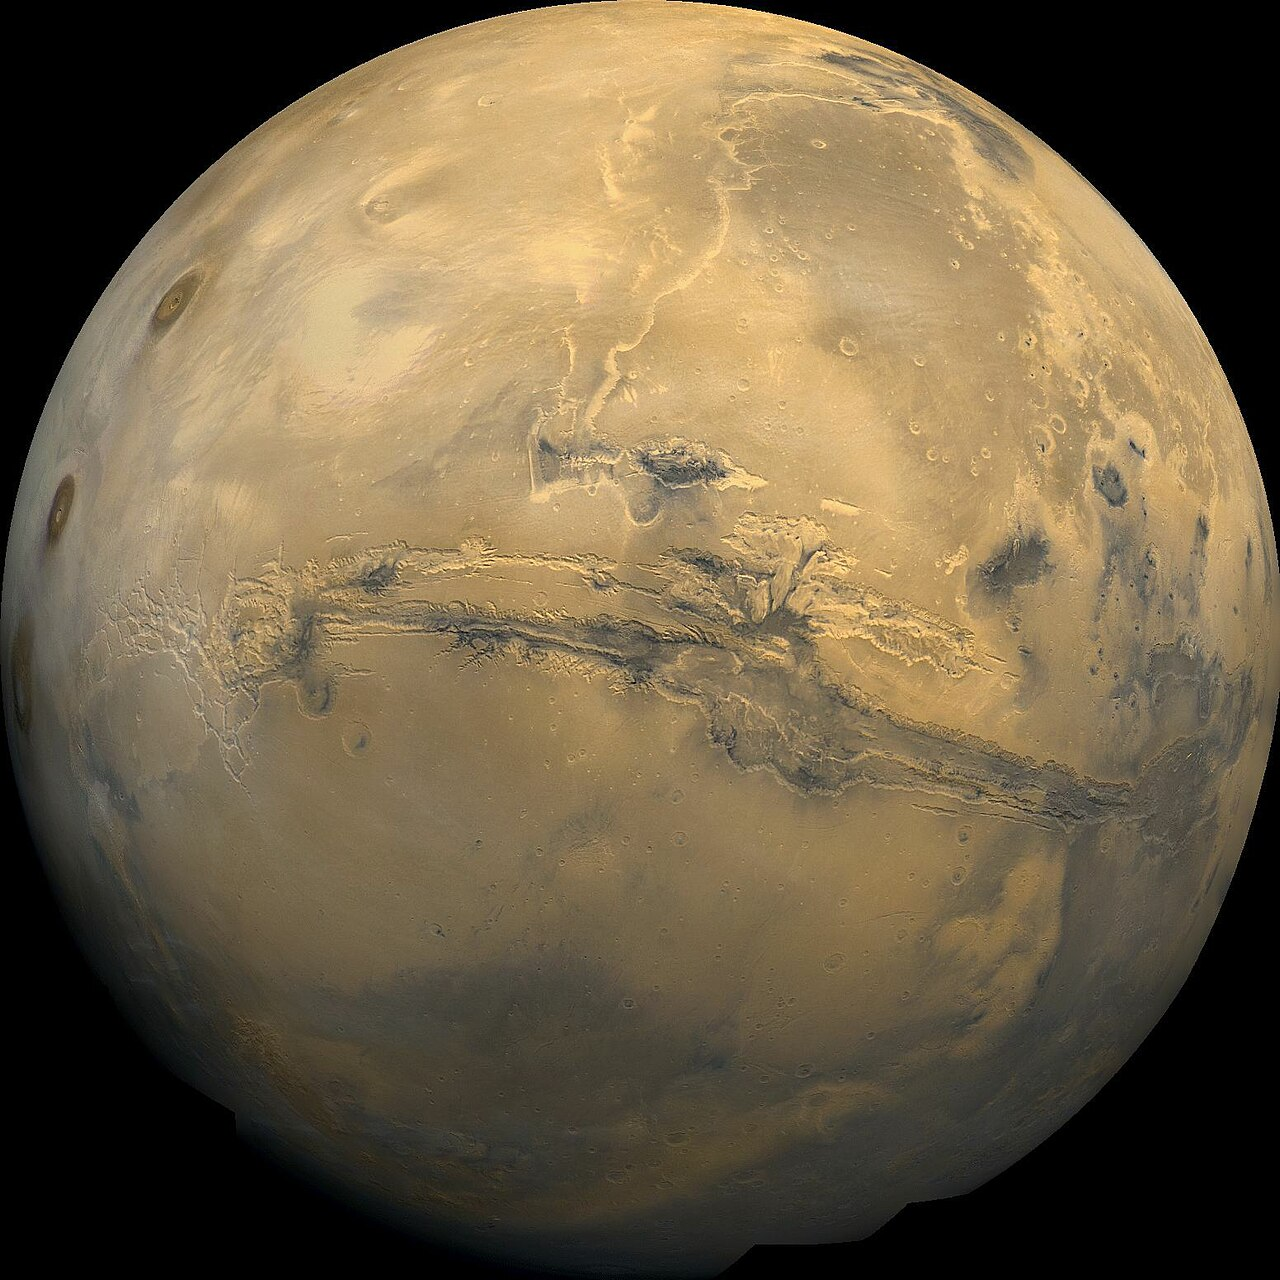
\includegraphics[height=1.75cm]{images/book1/mars.jpg} \\
{\footnotesize Mercurius} & {\footnotesize Venus} &
{\footnotesize Aarde} & {\footnotesize Mars} \\[4pt]
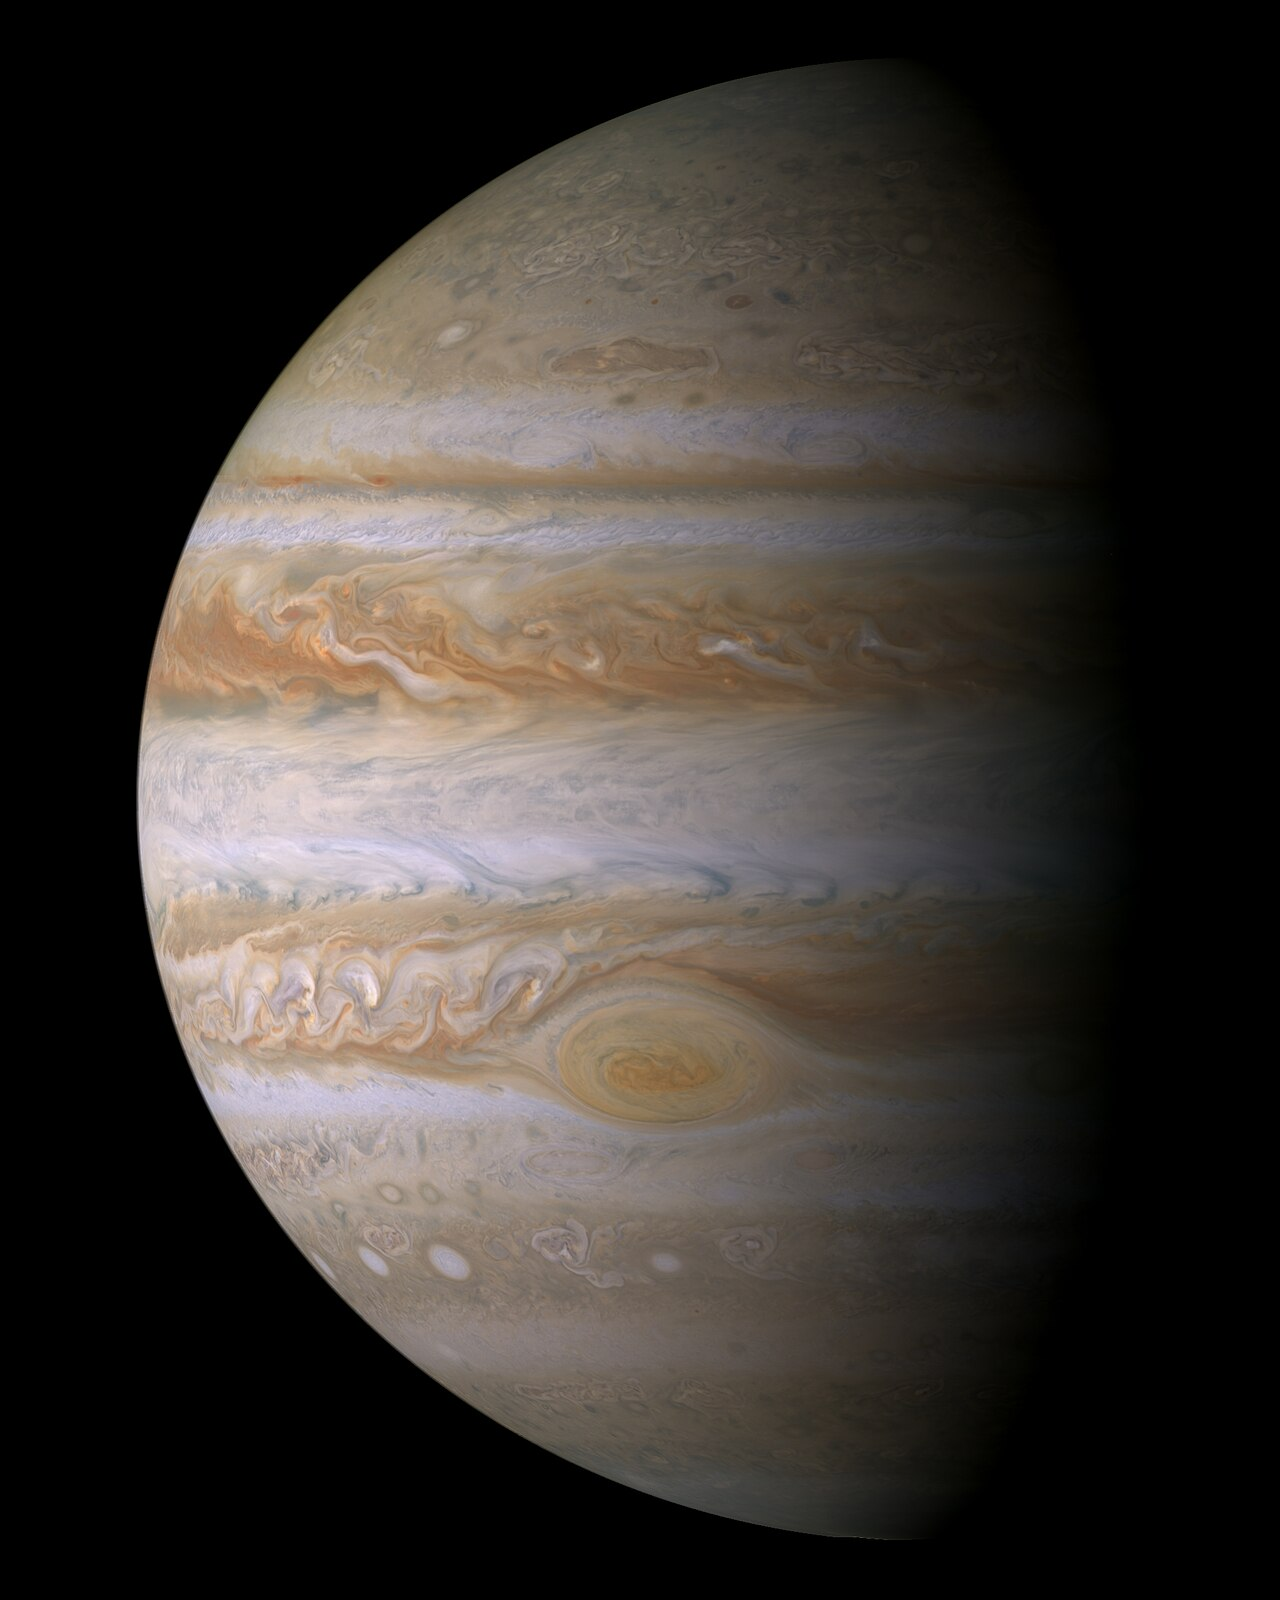
\includegraphics[height=1.75cm]{images/book1/jupiter.jpg} &
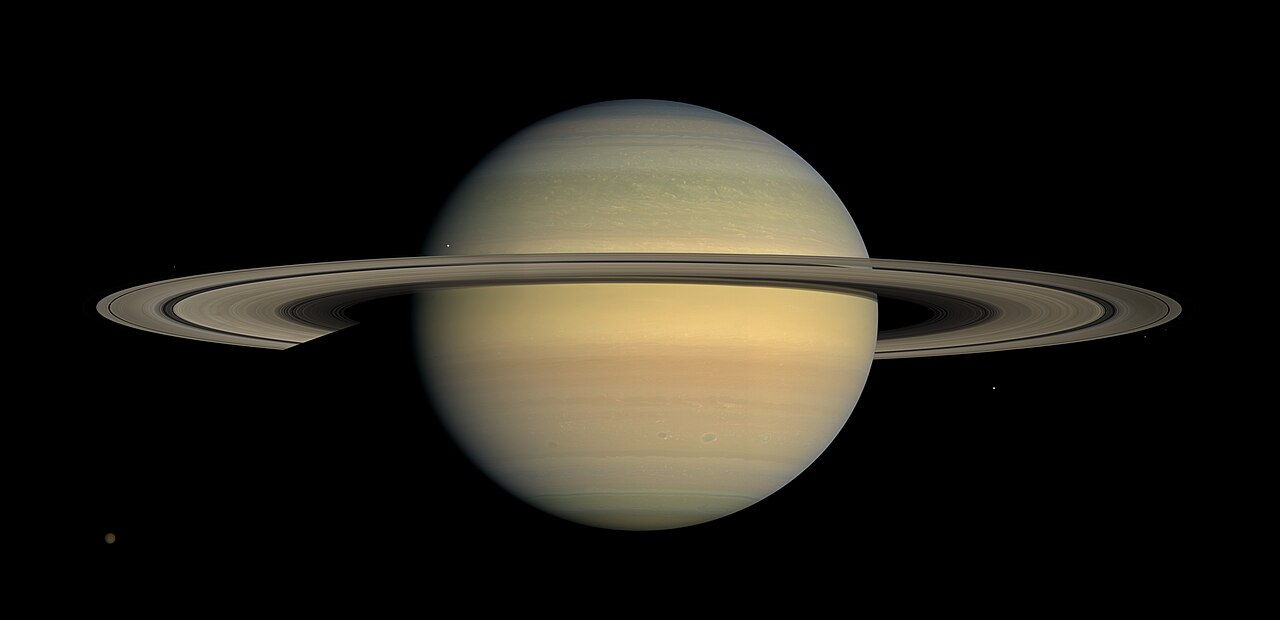
\includegraphics[height=1.75cm]{images/book1/saturn.jpg} &
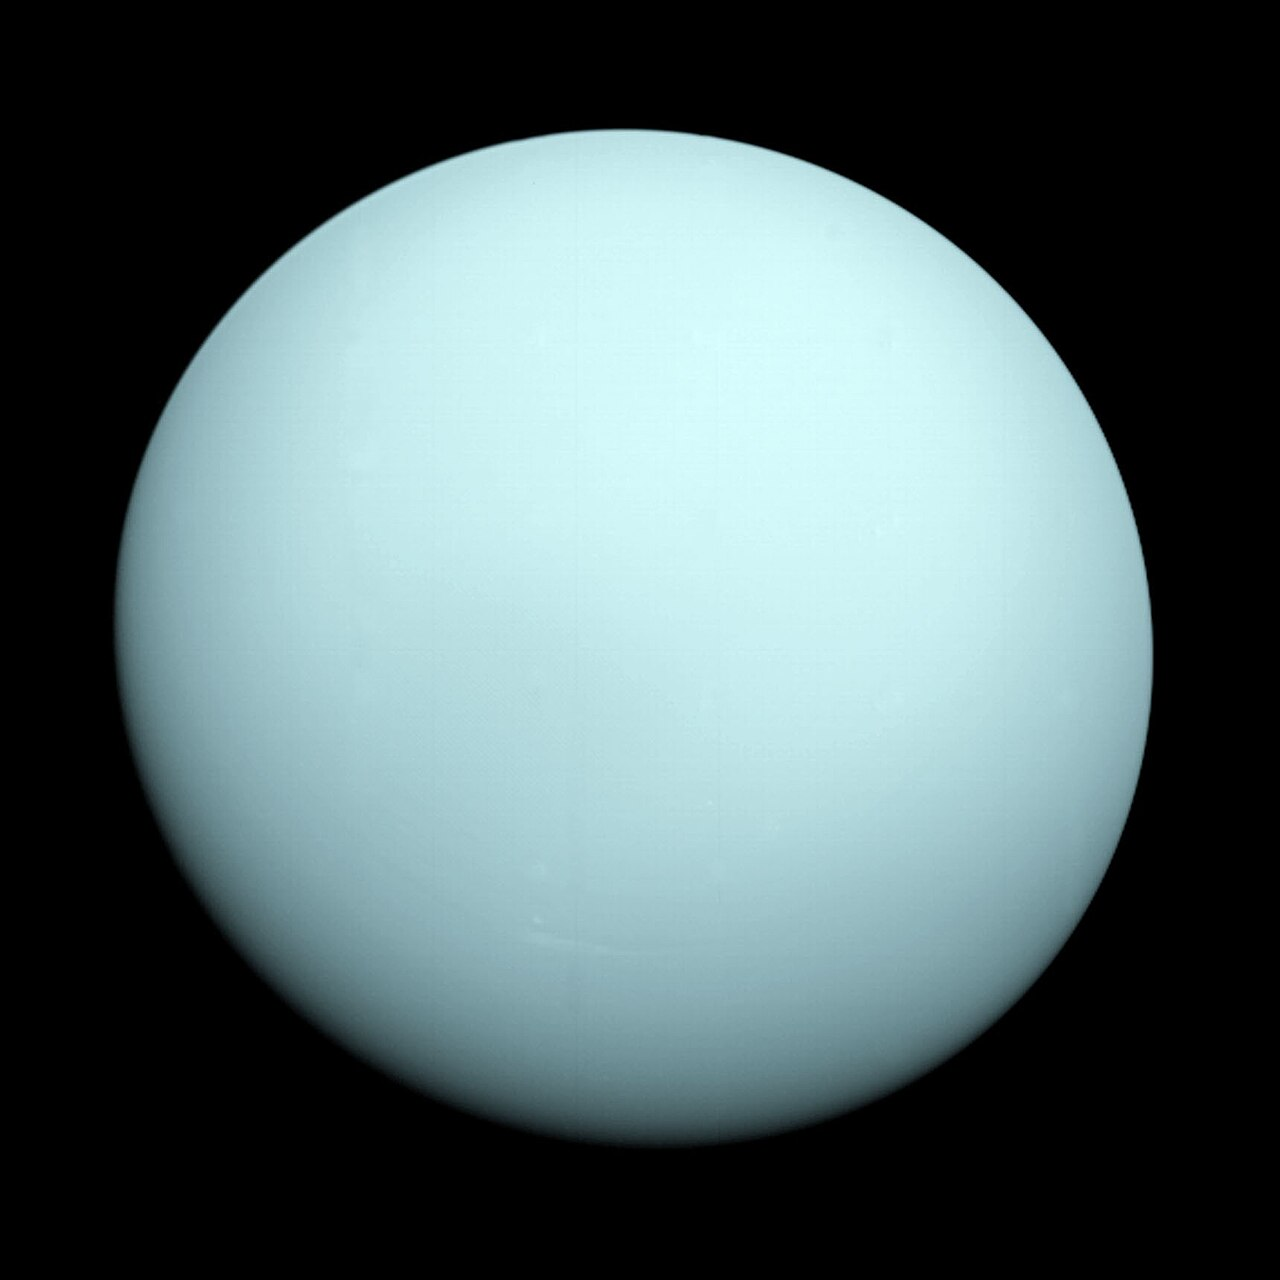
\includegraphics[height=1.75cm]{images/book1/uranus.jpg} &
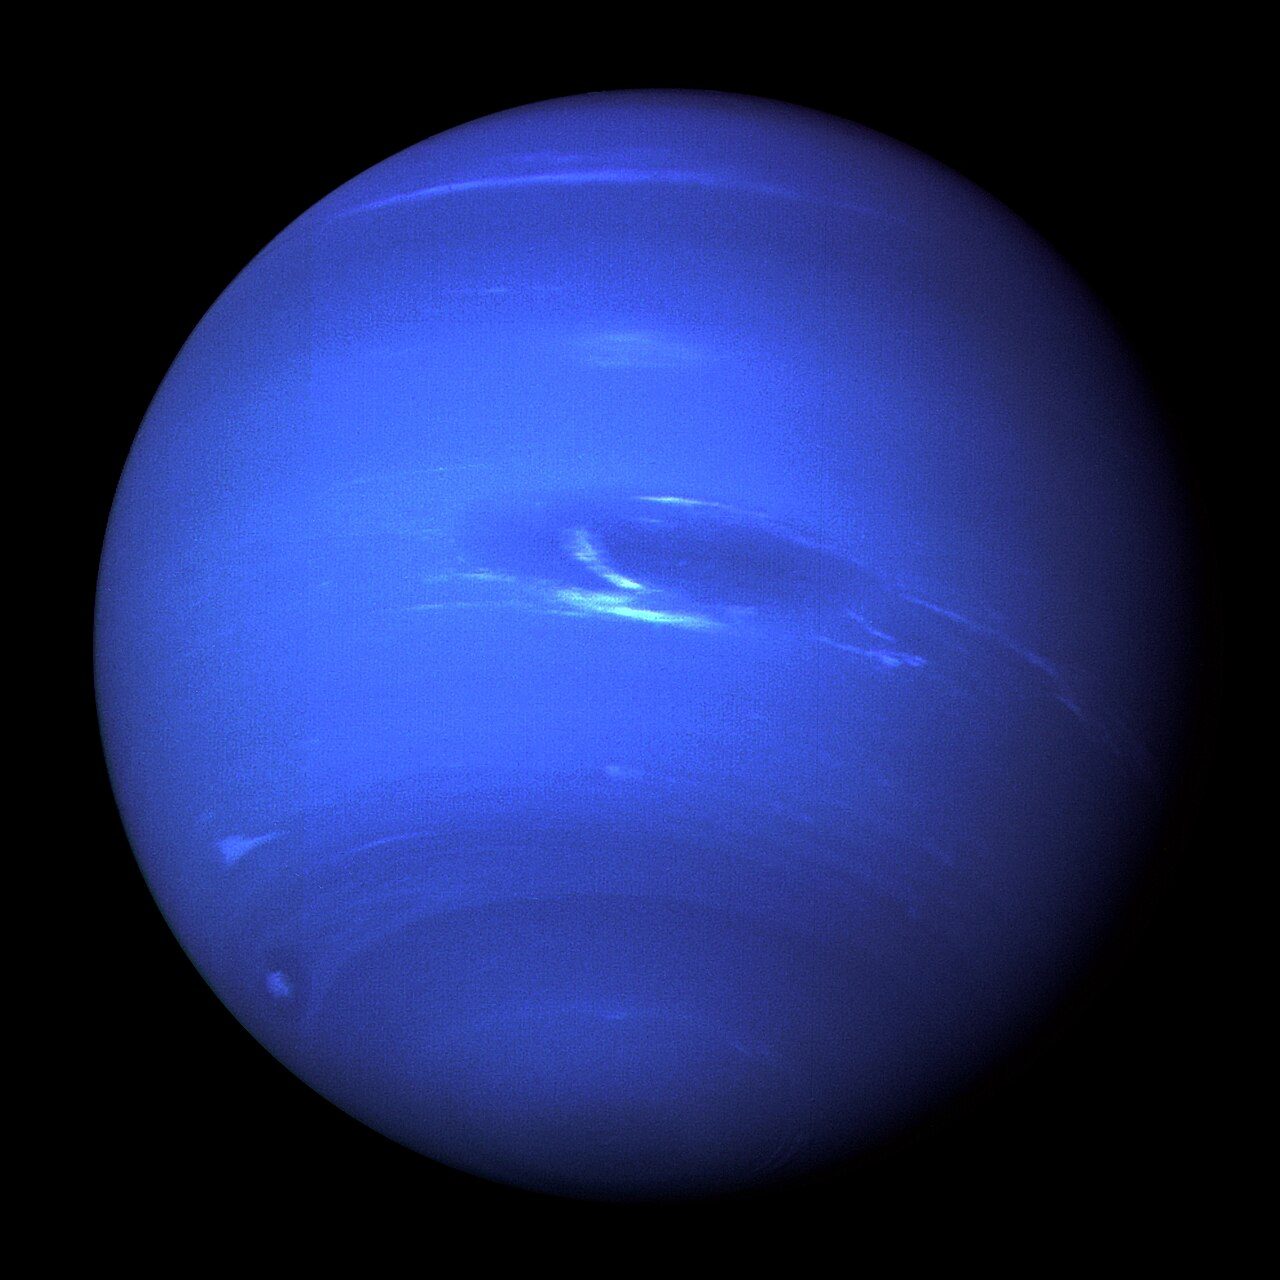
\includegraphics[height=1.75cm]{images/book1/neptune.jpg} \\
{\footnotesize Jupiter} & {\footnotesize Saturnus} &
{\footnotesize Uranus} & {\footnotesize Neptunus}
\end{tabular}

{\small De echte gezichten van de Zon en haar acht planeten,
gefotografeerd door ruimtesondes (groottes en afstanden niet op
schaal; Venus is als radarkaart afgebeeld --- haar wolken verbergen de
grond). \emph{Foto's: NASA (publiek domein).}}
\end{omfigure}

\begin{example}[Manen zijn geen planeten]\label{ex:g4:solar-system:moons}
Onze \omterm{def:g2:moon-in-the-sky:moon}{Maan} cirkelt om de \emph{Aarde}, niet rechtstreeks om de Zon ---
dus is ze geen \omterm{def:g4:solar-system:planet}{planeet} maar een \emph{maan}, een metgezel van een
\omterm{def:g4:solar-system:planet}{planeet}. Andere planeten hebben hun eigen manen: Mars heeft er twee
kleine, Jupiter en Saturnus elk tientallen. Een maan hoort bij haar
\omterm{def:g4:solar-system:planet}{planeet}; de \omterm{def:g4:solar-system:planet}{planeet} hoort bij de Zon.
\end{example}

\section{Hoe ver is ver}

\begin{method}[Een schaalmodel van het zonnestelsel]\label{met:g4:solar-system:model}
De afstanden tussen planeten zijn enorm --- miljoenen kilometers. Om
ze te voelen, bouw je in een park een schaalmodel van het
\omterm{def:g4:solar-system:family}{zonnestelsel}, waarbij je elke grootte en elke afstand met dezelfde
factor verkleint:
\begin{enumerate}
  \item laat de Zon een voetbal zijn die bij het hek ligt;
  \item dan is de Aarde een peperkorrel --- en om haar eerlijk neer
        te leggen, loop je ongeveer $30$ grote stappen van de voetbal
        vandaan;
  \item Mercurius, een speldenknop, staat ongeveer $12$ stappen van
        de voetbal; Jupiter, een knikker, ongeveer $150$ stappen;
        Neptunus, een klein kraaltje, ongeveer $900$ stappen ---
        bijna een kilometer verderop!
\end{enumerate}
Loop het uit, en voel wat geen tekening laat zien: het
\omterm{def:g4:solar-system:family}{zonnestelsel} is bijna helemaal lege ruimte, met piepkleine werelden
heel ver uit elkaar. In dit model staat één grote stap voor ongeveer
vijf miljoen kilometer echte ruimte.
\end{method}

\begin{omfigure}
\begin{tikzpicture}[scale=0.85]
  \draw[-Stealth, thick] (0,0) -- (11.2,0);
  \fill[omThm] (0.5,0) circle (0.3);
  \node[below, font=\footnotesize] at (0.5,-0.42) {voetbal};
  \fill[omDef] (1.6,0) circle (0.05);
  \draw[omExo, very thin] (1.6,-0.18) -- (1.6,-0.85);
  \node[below, font=\footnotesize] at (1.6,-0.88) {speldenknop};
  \fill[omDef] (3.2,0) circle (0.08);
  \node[below, font=\footnotesize] at (3.2,-0.35) {peperkorrel (Aarde)};
  \fill[omDef] (6.0,0) circle (0.16);
  \draw[omExo, very thin] (6.0,-0.24) -- (6.0,-0.85);
  \node[below, font=\footnotesize] at (6.0,-0.88) {knikker (Jupiter)};
  \fill[omDef] (10.6,0) circle (0.1);
  \node[below, font=\footnotesize] at (10.6,-0.38) {kraaltje (Neptunus)};
  \node[above, font=\small] at (5.6,0.5)
    {$12$ stappen, $30$ stappen, $150$ stappen, $900$ stappen\dots};
\end{tikzpicture}

{\small Het schaalmodel: krimp de Zon tot een voetbal, en het hele
\omterm{def:g4:solar-system:family}{zonnestelsel} past in een park --- maar net.}
\end{omfigure}

\begin{example}[De dwalers aan onze hemel]\label{ex:g4:solar-system:wanderers}
Venus is vaak de eerste ``\omterm{def:g4:solar-system:star}{ster}'' van de avond, laaiend in het westen
na \omterm{def:g1:day-and-night:daynight}{zonsondergang} --- zo helder omdat ze onze naaste buur is,
gehuld in witte wolken die het zonlicht rijkelijk terugsturen. Mars
gloeit zwak oranje; Jupiter en Saturnus schijnen rustig en helder.
Volg er een paar weken lang een tegen de vaste sterren: hij dwaalt
weg --- precies het dwalen dat planeten hun oude naam gaf.
\end{example}

\begin{remark}[Een oud plaatje, hertekend]\label{rem:g4:solar-system:history}
Het grootste deel van de geschiedenis zetten mensen de Aarde in het
midden van alles, met Zon, \omterm{def:g2:moon-in-the-sky:moon}{Maan} en planeten die om ons heen
cirkelden. Zorgvuldige waarnemers van de dwalers merkten dat dat
plaatje kraakte --- planeten dwalen soms een tijdje
\emph{achteruit}, moeilijk te verklaren met de Aarde op de troon in
het midden. Het zonsgerichte plaatje dat je zojuist hebt geleerd,
verklaarde die dwaaltochten eenvoudig, en het hoort bij de
gedurfdste ideeën die mensen ooit hebben aanvaard: ons thuis is niet
het middelpunt --- het is de derde \omterm{def:g4:solar-system:planet}{planeet} vanaf de Zon.
\end{remark}

\section{Oefeningen}

\begin{exercise}[$\star$]\label{exo:g4:solar-system:1}
Wat is het verschil tussen een \omterm{def:g4:solar-system:star}{ster} en een \omterm{def:g4:solar-system:planet}{planeet}? Wat is de Zon?
En de Aarde?
\end{exercise}

\begin{exercise}[$\star$]\label{exo:g4:solar-system:2}
Noem de acht planeten op volgorde vanaf de Zon. Welke is de onze?
\end{exercise}

\begin{exercise}[$\star$]\label{exo:g4:solar-system:3}
Welke planeten zijn klein en rotsachtig? Welke zijn de gasreuzen?
Noem de allergrootste, en die met de beroemde ringen.
\end{exercise}

\begin{exercise}[$\star$]\label{exo:g4:solar-system:4}
Waarom telt de \omterm{def:g2:moon-in-the-sky:moon}{Maan} niet mee bij de planeten? Waar cirkelt ze
omheen?
\end{exercise}

\begin{exercise}[$\star$]\label{exo:g4:solar-system:5}
Mercurius doet $88$ dagen over een ronde om de Zon, de Aarde $365$,
Neptunus $165$ jaar. Welke gewoonte van de planeten laten deze
getallen zien?
\end{exercise}

\begin{exercise}[$\star$]\label{exo:g4:solar-system:6}
Wat speelt in het schaalmodel in het park de Zon, en hoeveel stappen
verderop staat de Aarde? Waaruit bestaat het \omterm{def:g4:solar-system:family}{zonnestelsel} qua ruimte
bijna helemaal?
\end{exercise}

\begin{exercise}[$\star$]\label{exo:g4:solar-system:7}
Venus schittert schitterend, en toch is ze geen \omterm{def:g4:solar-system:star}{ster}. Waar komt haar
\omterm{def:g1:light-and-shadows:source}{licht} vandaan? (Een oude bekende geeft het antwoord: denk aan de
\omterm{def:g2:moon-in-the-sky:moon}{Maan}.)
\end{exercise}

\begin{exercise}[$\star$]\label{exo:g4:solar-system:8}
Hoe kun je door een paar weken naar de hemel te kijken zien dat een
helder lichtje een \omterm{def:g4:solar-system:planet}{planeet} is en geen \omterm{def:g4:solar-system:star}{ster}?
\end{exercise}

\begin{exercise}[$\star$]\label{exo:g4:solar-system:9}
In het parkmodel staat Jupiter op ongeveer $150$ stappen en de Aarde
op ongeveer $30$. Ruwweg hoeveel keer verder van de Zon staat Jupiter
dan de Aarde?
\end{exercise}

\begin{exercise}[$\star\star$]\label{exo:g4:solar-system:10}
Een vriend tekent het \omterm{def:g4:solar-system:family}{zonnestelsel} met alle acht planeten dicht
opeengepakt rond de Zon, zoals de eerste tekening van dit hoofdstuk,
en vraagt waarom sondes er jaren over doen om de buitenste
planeten te bereiken. Zet hem recht met het schaalmodel in het park
--- waarover liegen bijna alle tekeningen van het
\omterm{def:g4:solar-system:family}{zonnestelsel}, en waarom moeten ze dat wel?
\end{exercise}

\begin{exercise}[$\star\star$]\label{exo:g4:solar-system:11}
Toen men geloofde dat de Aarde in het midden van alles stond, welk
raadsel aan de hemel kraakte er tegen dat plaatje? Hoe loste het
plaatsen van de Zon in het midden het raadsel op --- en wat kostte het
nieuwe portret ons aan trots?
\end{exercise}
